%%
%% bioq -- Bioinformatics (Applications Note) -- Supplementary Information (LaTeX)
%%
%% Standalone render of the supplementary figures/tables for the bioq manuscript.
%% Unlike ../manuscript.tex it deliberately does NOT use oup-authoring-template.cls:
%% supplementary material is a plain, separately-uploaded PDF, not journal-copy,
%% so a standard single-column article layout is simpler and dependency-free.
%% It keeps the author--year reference style (natbib + oup-abbrvnat.bst) so the
%% SI bibliography reads the same as the main text.
%%

\documentclass[11pt]{article}

\usepackage[a4paper,margin=25mm]{geometry}
\usepackage[T1]{fontenc}
\usepackage{textcomp}
\usepackage{graphicx}
\usepackage[font=small,labelfont=bf]{caption}
\usepackage[authoryear,round]{natbib}
\usepackage{array}
\usepackage{booktabs}
\usepackage{longtable}

%% Figures live one level up, in paper-bioinformatics/figures/.
\graphicspath{{../figures/}}

\begin{document}

\begin{center}
{\LARGE\bfseries Supplementary Information}\\[6pt]
{\large bioq: a unified, agent-native gateway to a fleet of AI drug-discovery methods}
\end{center}

\vspace{2\baselineskip}

%% ---------------------------------------------------------------------------
%% Number the supplementary figures S1, S2, ... (do not continue the main
%% figure counter from the parent manuscript), so ``Figure S1''--``Figure S9''
%% references in the main text stay correct.
%% ---------------------------------------------------------------------------
\setcounter{figure}{0}
\renewcommand{\thefigure}{S\arabic{figure}}
%% Supplementary tables are likewise numbered S1, S2, ... independently of the
%% parent manuscript, so the Table S1 / Table S2 references stay correct.
\setcounter{table}{0}
\renewcommand{\thetable}{S\arabic{table}}

\section*{Supplementary figures}

\begin{figure}[!ht]
\centering
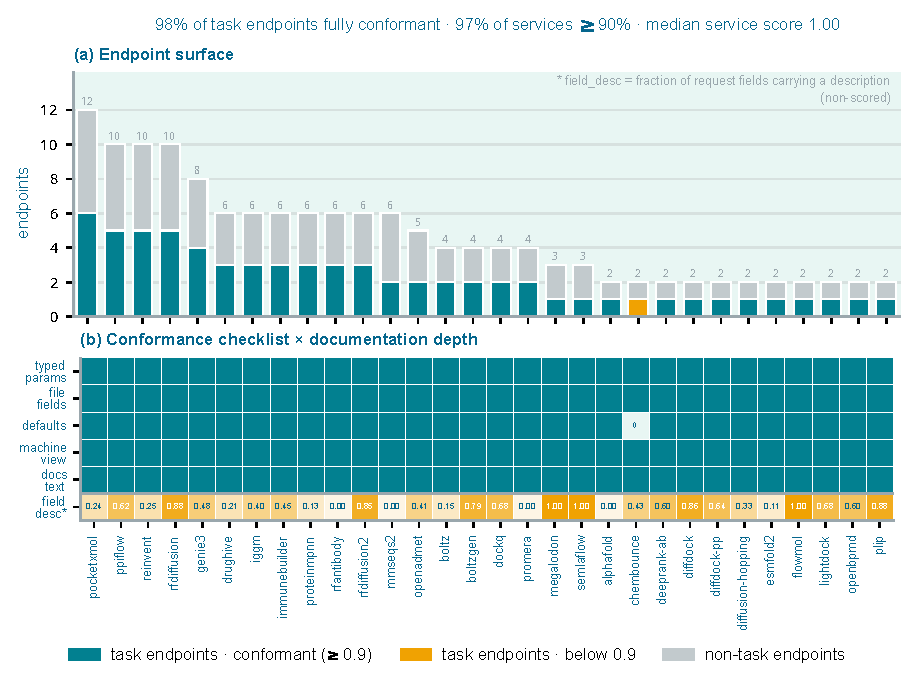
\includegraphics[width=\textwidth,height=0.85\textheight,keepaspectratio]{suppfig_s1_conformance}
\caption{Fleet-wide audit of the uniform, self-describing contract. A
  manifest-only audit of the 30 deployed services (141 endpoints, 68
  of them \texttt{bioq run} task endpoints) scores every endpoint
  against a five-item checklist --- the structural items
  \texttt{typed\_params}, \texttt{file\_fields}, and
  \texttt{machine\_view}, and the metadata items \texttt{defaults} and
  \texttt{docs\_text}. 98.5\,\% of task endpoints are fully conformant
  and 96.7\,\% of services sit at or above a 0.9 score (median 1.0);
  the single residual gap is one unannotated
  \texttt{input\_smiles\_uri} default on \texttt{chembounce}
  \texttt{scaffold\_hop}, which falls below the bar (amber).  (a)
  Endpoint surface, per service. Each vertical bar is a service's
  total endpoint count --- a dark base for task (async job interface)
  endpoints and a light top for non-task (sync job and status
  interface) endpoints. Teal marks services at or above the 0.9 bar;
  amber marks those below it.  (b) Conformance checklist $\times$
  documentation depth. One column per service and one row per contract
  item. The five scored rows report the fraction of task endpoints
  passing each checklist item; the final \texttt{field\_desc} row
  (non-scored) reports the mean fraction of request fields carrying a
  description.}
\label{fig:s1}
\end{figure}

\begin{figure}[!ht]
\centering
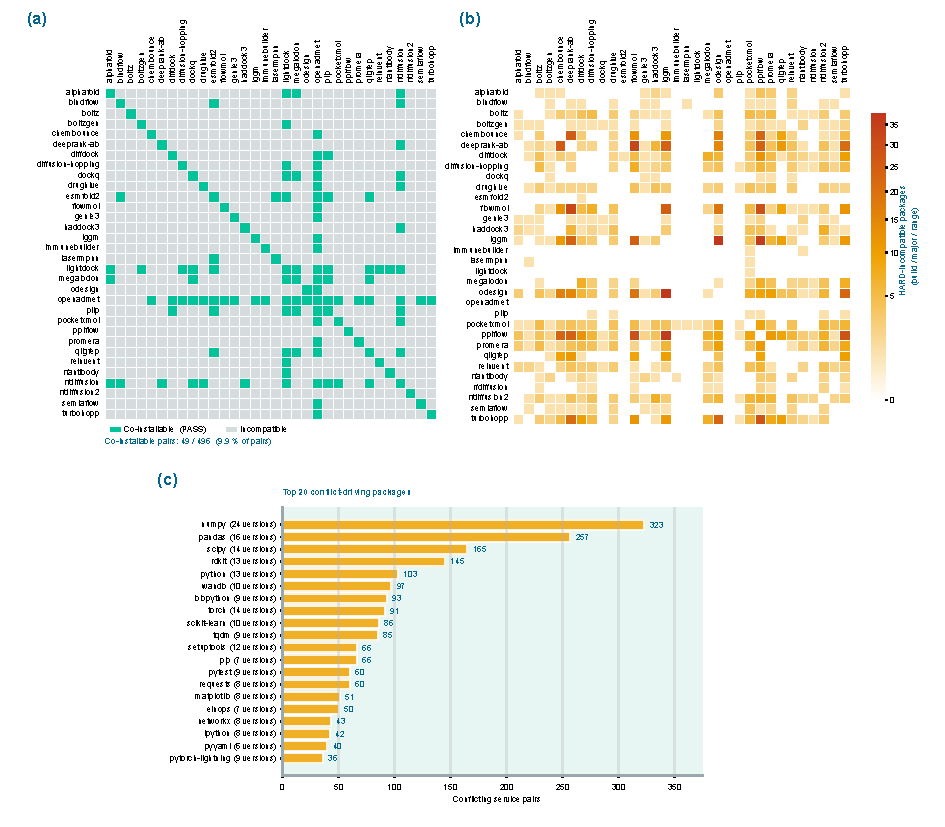
\includegraphics[width=\textwidth,height=0.85\textheight,keepaspectratio]{suppfig_s2_incompatibility}
\caption{Declared-dependency incompatibility of the bioq fleet (the 32 tools with
parseable upstream dependency specifications; 496 pairs).
(a) Co-installability: whether two tools' declared dependencies can literally
share one environment as-is (green = co-installable, grey = not; 49 of 496 pairs,
9.9\,\%).
(b) HARD-conflict heatmap: disjoint version ranges per tool pair --- no single
version satisfies both.
(c) Top 20 conflict-driving packages.}
\label{fig:s2}
\end{figure}

\begin{figure}[!ht]
\centering
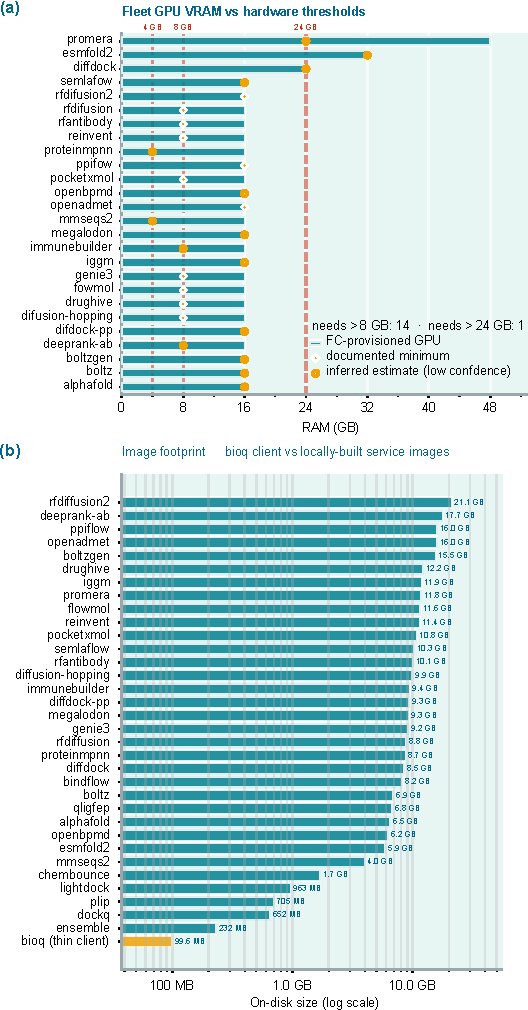
\includegraphics[width=\textwidth,height=0.85\textheight,keepaspectratio]{suppfig_s3_access_barrier}
\caption{Compute barrier for the full services fleet.  (a) GPU VRAM
  consumption per service. VRAM requirements marked as inferred are
  best-known estimates (15 of 26). The fleet cannot run on laptop
  GPUs.  (b) Storage footprint of the bioq client and service Docker
  images (model weights excluded from Docker images).}
\label{fig:s3}
\end{figure}

\begin{figure}[!ht]
\centering
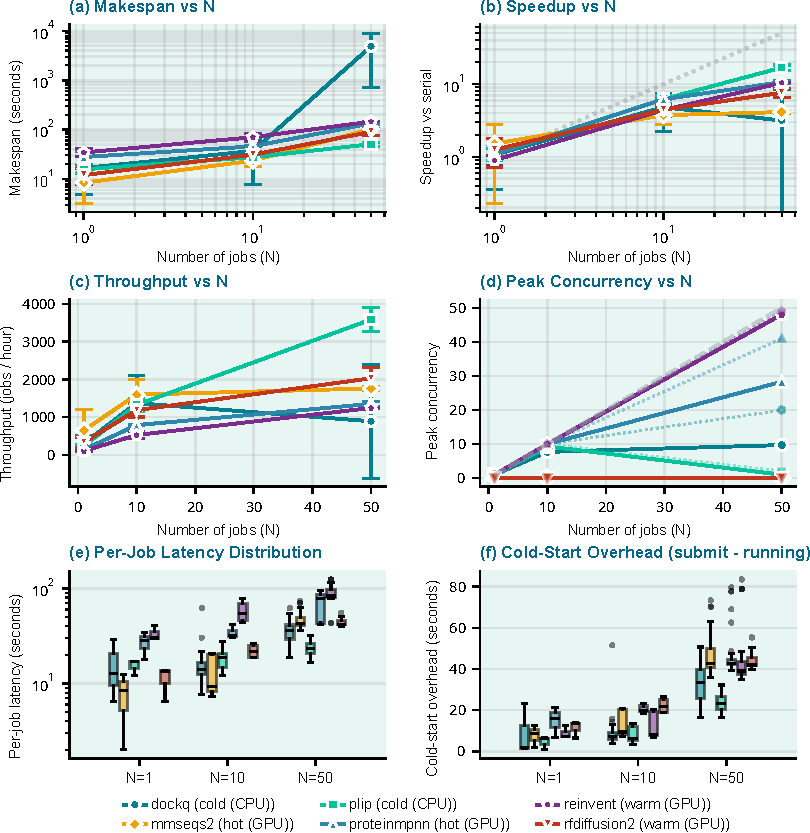
\includegraphics[width=\textwidth,height=0.85\textheight,keepaspectratio]{suppfig_s4_concurrency}
\caption{Throughput scaling of bioq serverless fan-out on
Alibaba Cloud Function Compute (FC). Six representative services spanning three serverless
tiers --- cold CPU (\texttt{dockq}, \texttt{plip}), hot GPU (\texttt{mmseqs2},
\texttt{proteinmpnn}), and warm GPU (\texttt{reinvent}, \texttt{rfdiffusion2}) ---
are measured as a function of batch size $N \in \{1, 10, 50\}$; the upper bound
$N = 50$ is the FC GPU instance-quota ceiling. Each point is the mean over three
independent replicates, with error bars showing $\pm$1 standard deviation. Colour
and marker identify the service (shared legend beneath the panels).
(a) Makespan vs $N$ (log--log), wall-clock to finish all N jobs; (b) Speedup vs $N$ (log--log), $N \times$ single-job time / makespan, relative to the
serial baseline; (c) Throughput vs $N$, completed jobs / makespan; (d) Peak concurrency vs $N$, max simultaneous worker instances observed; (e) Per-job
latency distribution (log-scale box plots), wall-clock time for a single job from submit to completion; (f) Cold-start overhead (box plots), time from submit to first running status.}
\label{fig:s4}
\end{figure}

\begin{figure}[!ht]
\centering
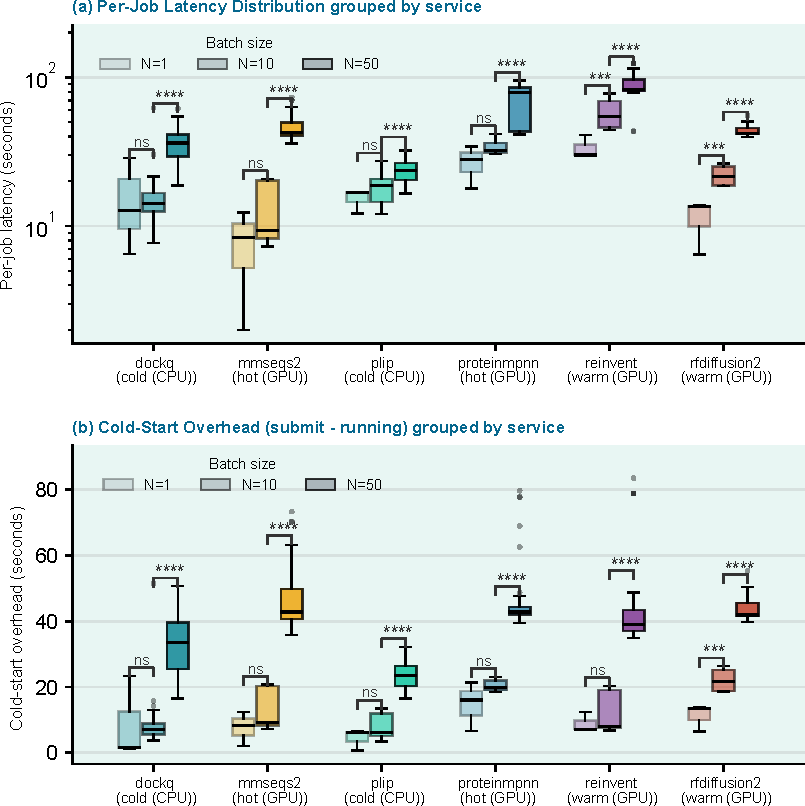
\includegraphics[width=\textwidth,height=0.85\textheight,keepaspectratio]{suppfig_s5_concurrency_by_services}
\caption{Per-job latency and cold-start overhead, grouped by
service, on FC. The x-axis lists six services; within each
service, three box plots show batch size $N = 1, 10, 50$ (lighter $\rightarrow$
darker). Boxes pool all jobs across three replicates. Brackets show two-sided
Mann--Whitney U tests between adjacent $N$ levels.
(a) Per-job latency (seconds, y-axis log scale);
(b) Cold-start overhead (seconds).}
\label{fig:s5}
\end{figure}

\begin{figure}[!ht]
\centering
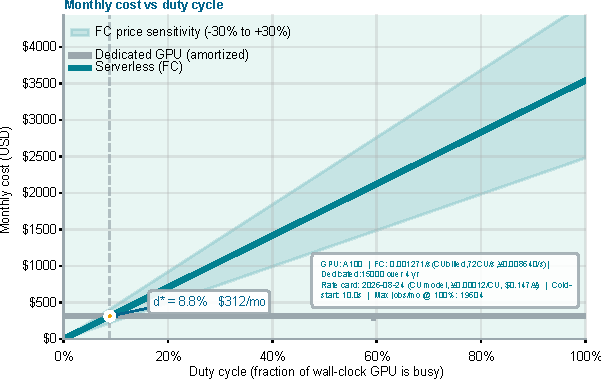
\includegraphics[width=\textwidth,height=0.85\textheight,keepaspectratio]{suppfig_s6_cost}
\caption{ Monthly cost and duty-cycle break-even for serverless and
  dedicated A100-class GPU capacity.  The bioq serverless estimate
  uses the Alibaba Cloud Function Compute pricing schedule
  (2026). Under the first pricing tier, a 40-GB Ampere-class
  allocation consumes 72~CU\,s$^{-1}$ at CNY~0.00012 per CU,
  equivalent to USD~4.57\,h$^{-1}$ at USD~1 = CNY~6.80. The
  calculation includes 10\,s of billed cold-start overhead per
  invocation and yields a weighted mean cost of approximately USD~0.18
  per observed job. The owned-A100 comparison assumes a purchase price
  of USD~15,000 amortized over four years (USD~0.43\,h$^{-1}$),
  whereas the persistent cloud-VM comparison assumes
  USD~2.50\,h$^{-1}$. The resulting break-even duty cycles are
  approximately 8.8\,\% and 52\,\%, respectively; below each
  crossover, serverless execution is less expensive. The shaded band
  shows the price-sensitivity sweep. The ownership estimate excludes
  host-system, electricity, cooling, maintenance, financing, storage,
  and network-transfer costs and is therefore conservative in favor of
  owned hardware.  }
\label{fig:s6}
\end{figure}


\begin{figure}[!ht]
\centering
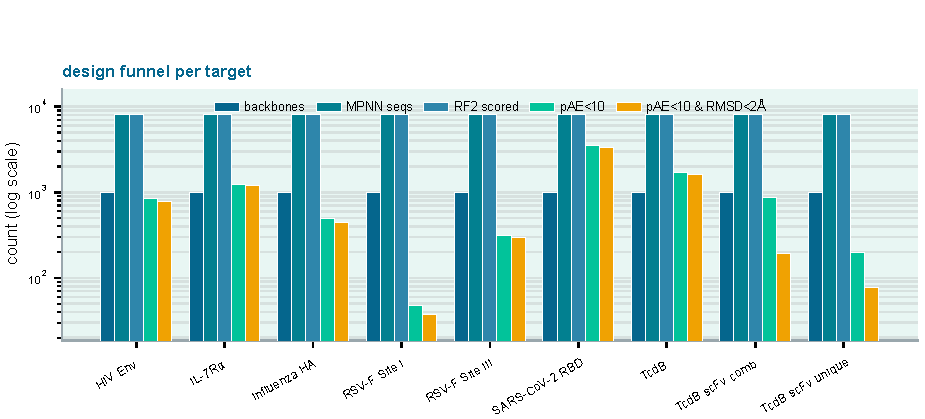
\includegraphics[width=\textwidth,height=0.85\textheight,keepaspectratio]{suppfig_s7_rfantibody_funnel}
\caption{Per-target design funnel for the nine-target
RFantibody de novo antibody-design campaign run entirely through bioq (three
\texttt{bioq run} calls per target, no local GPU). For each target, five grouped
vertical bars report the count at successive pipeline stages: RFdiffusion
backbones (1{,}000), ProteinMPNN sequences (8{,}000 = 8 sequences per backbone),
sequences carried through RF2 structure prediction and scoring (8{,}000), designs
passing the interface-pAE $<$ 10 filter, and designs passing the combined
acceptance criterion (interface pAE $<$ 10 \emph{and} design--model CDR RMSD
$<$ 2 \AA{}, self-consistency RMSD, design vs RF2-predicted structure; amber). The y-axis is log-scaled.}
\label{fig:s7}
\end{figure}

\begin{figure}[!ht]
\centering
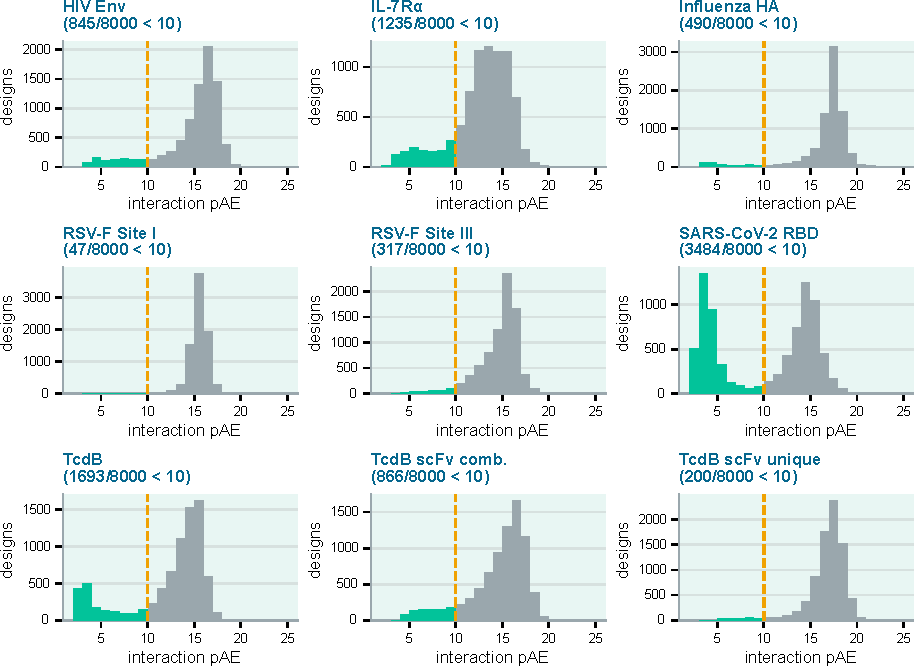
\includegraphics[width=\textwidth,height=0.85\textheight,keepaspectratio]{suppfig_s8_rfantibody_pae}
\caption{Distribution of interface pAE
(\texttt{interaction\_pae}, a.k.a.\ \texttt{pae\_interaction} in the paper) across
all 8{,}000 designs per target, one histogram per target in a 3$\times$3 grid.
Green bars mark designs passing the pAE $<$ 10 filter, grey bars the failures, and
the dashed amber line the threshold. All panels share a single binning (2--26 in
unit steps); each panel title reports the pass count over the total.}
\label{fig:s8}
\end{figure}

\begin{figure}[!ht]
\centering
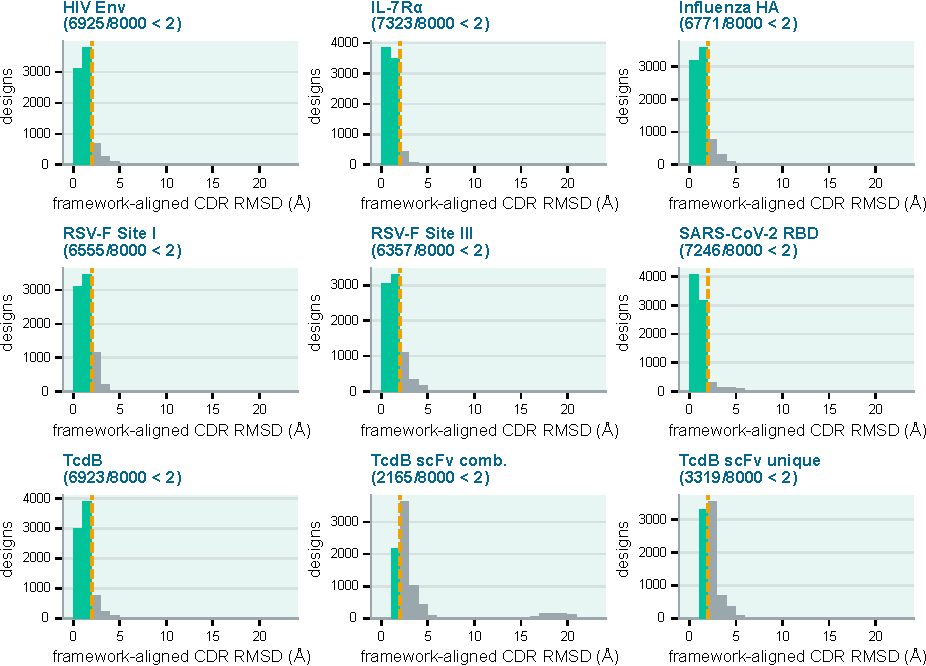
\includegraphics[width=\textwidth,height=0.85\textheight,keepaspectratio]{suppfig_s9_rfantibody_rmsd}
\caption{Distribution of design--model CDR RMSD across all 8{,}000
designs per target, one histogram per target in a 3$\times$3 grid. Green bars mark
designs passing the RMSD $<$ 2 \AA{} filter, grey bars the failures, and the dashed
amber line the 2 \AA{} threshold. All panels share a single binning (0--24 \AA{} in
1 \AA{} steps).}
\label{fig:s9}
\end{figure}


\clearpage
\section*{Supplementary Tables}

\begin{footnotesize}
\setlength{\tabcolsep}{5pt}
\begin{longtable}{@{}>{\raggedright\arraybackslash}p{25mm}>{\raggedright\arraybackslash}p{26mm}>{\raggedright\arraybackslash}p{28mm}>{\raggedright\arraybackslash}p{70mm}@{}}
\caption{The 38-service bioq fleet. Short names omit the \texttt{-server} suffix. Stages: 1 Structure prediction, 2 Sequence search, 3 De novo design, 4 Docking \& screening, 5 Affinity / free energy, 6 ADMET / PK, 7 Scoring \& QC. Modalities: protein, antibody/VHH, small molecule, peptide, nucleic acid, cross-modal. Citations are author--year.}
\label{tab:s1}\\
\toprule
\textbf{Short name} & \textbf{Stage} & \textbf{Modality} & \textbf{Upstream method (citation)} \\
\midrule
\endfirsthead
\multicolumn{4}{@{}l}{\emph{Table S1 (continued)}}\\
\toprule
\textbf{Short name} & \textbf{Stage} & \textbf{Modality} & \textbf{Upstream method (citation)} \\
\midrule
\endhead
\bottomrule
\multicolumn{4}{r@{}}{\emph{continued on next page}}\\
\endfoot
\bottomrule
\endlastfoot
\texttt{alphafold} & Structure prediction & protein / cross-modal & AlphaFold / AlphaFold-Multimer \citep{jumper_highly_2021,abramson_accurate_2024,evans_protein_2021} \\
\texttt{boltz} & Structure prediction & cross-modal & Boltz-2 \citep{passaro_boltz-2_2025,wohlwend_boltz-1_2024} \\
\texttt{esmfold2} & Structure prediction & protein / antibody/VHH & ESMFold2 \citep{lin_evolutionary-scale_2023} \\
\texttt{immunebuilder} & Structure prediction & antibody/VHH & ImmuneBuilder \citep{abanades_immunebuilder_2023} \\
\texttt{promera} & Structure prediction & protein / antibody/VHH & Promera \citep{jing_promera_2026} \\
\texttt{ensemble} & Structure prediction & antibody/VHH / protein & Multi-method ensemble (AlphaFold / ESMFold / Boltz / Promera) \\
\texttt{mmseqs2} & Sequence search & protein / cross-modal & MMseqs2 \citep{steinegger_mmseqs2_2017} \\
\texttt{diamond} & Sequence search & protein / cross-modal & DIAMOND \citep{buchfink_clustering_2026} \\
\texttt{rfdiffusion} & De novo design & protein & RFdiffusion \citep{watson_novo_2023} \\
\texttt{rfdiffusion2} & De novo design & protein & RFdiffusion2 \citep{ahern_atom-level_2026,krishna_generalized_2024} \\
\texttt{genie3} & De novo design & protein & Genie 3 \citep{lin_fast_2026} \\
\texttt{ppiflow} & De novo design & protein / antibody/VHH & PPIFlow \citep{yu_high-affinity_2026} \\
\texttt{boltzgen} & De novo design & protein / antibody/VHH / peptide & BoltzGen \citep{stark_boltzgen_2025} \\
\texttt{rfantibody} & De novo design & antibody/VHH & RFantibody (RFdiffusion + ProteinMPNN + RoseTTAFold-2) \citep{bennett_atomically_2026,watson_novo_2023,dauparas_robust_2022,baek_accurate_2021} \\
\texttt{iggm} & De novo design & antibody/VHH & IgGM \citep{wang_iggm_2025} \\
\texttt{odesign} & De novo design & protein / nucleic acid / small molecule & ODesign \citep{zhang_odesign_2025} \\
\texttt{proteinmpnn} & De novo design & protein & ProteinMPNN \citep{dauparas_robust_2022} \\
\texttt{lasermpnn} & De novo design & protein / small molecule & LASErMPNN (+ LigandMPNN) \citep{fry_zero-shot_2026,dauparas_robust_2022} \\
\texttt{flowmol} & De novo design & small molecule & FlowMol3 \citep{dunn_flowmol3_2025} \\
\texttt{semlaflow} & De novo design & small molecule & SemlaFlow \citep{irwin_semlaflow_2025} \\
\texttt{megalodon} & De novo design & small molecule & Megalodon \citep{reidenbach_applications_2025} \\
\texttt{reinvent} & De novo design & small molecule & REINVENT \citep{loeffler_reinvent_2024,blaschke_reinvent_2020} \\
\texttt{pocketxmol} & De novo design & small molecule & PocketXMol \citep{peng_unified_2026} \\
\texttt{drughive} & De novo design & small molecule & DrugHIVE \citep{weller_structure-based_2024} \\
\texttt{chembounce} & De novo design & small molecule & ChemBounce \citep{jang_chembounce_2025} \\
\texttt{diffusion\-hopping} & De novo design & small molecule & DiffHopp \citep{torge_diffhopp_2023} \\
\texttt{turbohopp} & De novo design & small molecule & TurboHopp \citep{yoo_turbohopp_2024} \\
\texttt{diffdock} & Docking \& screening & small molecule & DiffDock \citep{corso_diffdock_2023} \\
\texttt{diffdock-pp} & Docking \& screening & protein & DiffDock-PP \citep{ketata_diffdock-pp_2023} \\
\texttt{lightdock} & Docking \& screening & protein & LightDock \citep{jimenez-garcia_lightdock_2018} \\
\texttt{haddock3} & Docking \& screening & protein / cross-modal & HADDOCK3 \citep{giulini_haddock3_2025} \\
\texttt{plip} & Docking \& screening & small molecule / protein & PLIP \citep{schake_plip_2025} \\
\texttt{bindflow} & Affinity / free energy & small molecule & BindFlow \citep{leon_bindflow_2026} \\
\texttt{qligfep} & Affinity / free energy & small molecule & QligFEP \citep{alencar_araripe_doing_2025} \\
\texttt{openbpmd} & Affinity / free energy & small molecule & OpenBPMD \citep{lukauskis_open_2022} \\
\texttt{openadmet} & ADMET / PK & small molecule & OpenADMET \citep{fraser_mapping_2026} \\
\texttt{dockq} & Scoring \& QC & protein & DockQ \citep{basu_dockq_2016,mirabello_dockq_2024} \\
\texttt{deeprank-ab} & Scoring \& QC & antibody/VHH & DeepRank-Ab \citep{xu_deeprank-ab_2025} \\
\bottomrule
\end{longtable}
\end{footnotesize}

% Structure prediction: AlphaFold \citep{jumper_highly_2021,abramson_accurate_2024},
% AlphaFold-Multimer \citep{evans_protein_2021}, RoseTTAFold
% \citep{baek_accurate_2021}, Boltz \citep{wohlwend_boltz-1_2024,passaro_boltz-2_2025},
% ESMFold \citep{lin_evolutionary-scale_2023}, ImmuneBuilder
% \citep{abanades_immunebuilder_2023}, Promera \citep{jing_promera_nodate}.

% De novo design: RFdiffusion \citep{watson_novo_2023}, Genie
% \citep{lin_fast_2026}, ProteinMPNN \citep{dauparas_robust_2022},
% REINVENT
% \citep{loeffler_reinvent_2024,blaschke_reinvent_2020}, FlowMol
% \citep{dunn_flowmol3_2025}, SemlaFlow \citep{irwin_semlaflow_2025}, Megalodon
% \citep{reidenbach_applications_2025}, PocketXMol \citep{peng_unified_2026}.

% Docking: DiffDock \citep{corso_diffdock_2023}, DiffDock-PP
% \citep{ketata_diffdock-pp_2023}, LightDock \citep{jimenez-garcia_lightdock_2018},
% HADDOCK3 \citep{giulini_haddock3_2025}, PLIP \citep{schake_plip_2025}.

% Affinity/free energy: BindFlow \citep{leon_bindflow_2026}, QligFEP
% \citep{alencar_araripe_doing_nodate}, OpenBPMD \citep{lukauskis_open_2022}.

% ADMET: OpenADMET \citep{fraser_mapping_2026}.

% Scoring: DockQ \citep{basu_dockq_2016,mirabello_dockq_2024}, DeepRank-Ab
% \citep{xu_deeprank-ab_2025}.



\begin{table}[!ht]
\centering
\footnotesize
\caption{Per-target in-silico design funnel for the nine-target RFantibody de novo
antibody-design campaign (seven VHH, two scFv), run entirely through bioq. Columns,
left to right: RFdiffusion backbones; ProteinMPNN sequences (eight per backbone);
sequences carried through RF2 folding and scoring; designs passing the interface-pAE
$<$ 10 filter; and designs passing the combined acceptance filter (interface pAE $<$ 10
\emph{and} design--model CDR RMSD $<$ 2 \AA{}). The final column reports the
published RFantibody per-target in-silico success rate for comparison. Targets are ordered by
the best-of-8 backbone pass rate.}
\label{tab:s2}
\setlength{\tabcolsep}{2pt}
\renewcommand{\arraystretch}{1.2}
\begin{tabular}{@{}>{\raggedright\arraybackslash}p{32mm} c r r r r r r r r@{}}
\toprule
\textbf{Target} & \textbf{Type} & \textbf{Backbones} & \textbf{Sequences} & \textbf{Scored} &
\textbf{\shortstack{pAE\\$<$10}} & \textbf{Passed} &
\textbf{\shortstack{Passed\\(\%)$^{\dagger}$}} &
\textbf{\shortstack{Best-of-8\\(\%)$^{\ddagger}$}} & \textbf{\shortstack{Published\\(\%)$^{\mathsection}$}} \\
\midrule
SARS-CoV-2 RBD & VHH & 1{,}000 & 8{,}000 & 8{,}000 & 3{,}484 & 3{,}321 & 41.51 & 70.6 & 28.0 \\
TcdB & VHH & 1{,}000 & 8{,}000 & 8{,}000 & 1{,}693 & 1{,}605 & 20.06 & 48.9 & 41.0 \\
IL-7R$\alpha$ & VHH & 1{,}000 & 8{,}000 & 8{,}000 & 1{,}235 & 1{,}200 & 15.00 & 43.0 & 34.5 \\
HIV Env & VHH & 1{,}000 & 8{,}000 & 8{,}000 & 845 & 781 & 9.76 & 34.2 & -- \\
RSV-F Site III & VHH & 1{,}000 & 8{,}000 & 8{,}000 & 317 & 293 & 3.66 & 17.2 & 25.0 \\
Influenza HA & VHH & 1{,}000 & 8{,}000 & 8{,}000 & 490 & 448 & 5.60 & 14.6 & 11.5 \\
RSV-F Site I & VHH & 1{,}000 & 8{,}000 & 8{,}000 & 47 & 37 & 0.46 & 2.4 & -- \\
\addlinespace
TcdB scFv (comb.) & scFv & 1{,}000 & 8{,}000 & 8{,}000 & 866 & 192 & 2.40 & 9.6 & -- \\
TcdB scFv (unique) & scFv & 1{,}000 & 8{,}000 & 8{,}000 & 200 & 77 & 0.96 & 5.8 & -- \\
\bottomrule
\end{tabular}
\par\medskip
\raggedright
$^{\dagger}$ Fraction of scored sequences passing the combined filter. $^{\ddagger}$
Fraction of backbones whose best-scoring of eight MPNN sequences passes the combined
filter; this per-backbone best-of-8 rate is the metric reported by the published
RFantibody method and gives the main-text pass-rate range.
$^{\mathsection}$ Published per-target in-silico success rate of the RFantibody method
\citep{bennett_atomically_2026}; a dash marks targets with no reported per-target
screening.
\end{table}

%% ---------------------------------------------------------------------------
%% Bibliography (author--year, matches the parent manuscript's oup-abbrvnat;
%% author lists truncated to 6 + "et al." by oup-abbrvnat-et-al.bst)
%% ---------------------------------------------------------------------------
\clearpage
\bibliographystyle{oup-abbrvnat-et-al}
\bibliography{references-escaped}

\end{document}
